\documentclass[aspectratio=169,8pt]{beamer}

\geometry{paperwidth=169mm,paperheight=95mm}

\usepackage[T1,T2A]{fontenc}
\usepackage[utf8]{inputenc}
\usepackage[main=russian,english]{babel}
\usepackage[normalem]{ulem}
\usepackage{hyperref}
\usepackage{amsmath,amsthm,amssymb,lmodern}
\usepackage{graphicx} % Allows including images
\usepackage{booktabs} % Allows the use of \toprule, \midrule and \bottomrule in tables
\usepackage{wrapfig}
\usepackage{caption}

\graphicspath{ {./images/} }

\usetheme{Boadilla}
\setbeamertemplate{caption}{\insertcaption}

\title[Проект по дисциплине МИИАД] {Проект по дисциплине "Методы искусственного интеллекта в анализе данных"}
\subtitle{Этап 2}

\author[Бобровских, Иванов, Угадяров] {Бобровских Глеб, Иванов Дмитрий, Угадяров Леонид \\ \tiny\url{https://github.com/ugadiarov-la-phystech-edu/aimda-project}}
\institute{Группа 4}


\begin{document}

\begin{frame}
\titlepage
\end{frame}

\begin{frame}
\frametitle{Набор данных и постановка задачи}

\begin{itemize}
\item { Рассматривается временной ряд количества убийств в США, совершённых за месяц, полученный агрегацией исходного набора данных Homicide Reports (1980-2014):\\https://www.kaggle.com/murderaccountability/homicide-reports }
\item Решается задача прогнозирования количества убийств на следующий месяц по историческим данным
\item Метрика качества --- \emph {RMSE} для значений временного ряда
\item {Актуальность --- качественное прогнозирование количества преступлений поможет эффективнее организовать работу полицейских учереждений  }
\end{itemize}

\begin{block}{Целевая переменная и признаки}
Целевая переменная: NumCases --- количество убийств на всей территории США за один месяц\\
Признаки: значения NumCases за предыдущие 12 месяцев и значения 117 агрегированных признаков исходного набора данных за предыдущие 12 месяцев (всего 1416 признаков)\\
Также производились эксперименты с использованием данных за предыдущие 24 месяца (2832 признака)
\end{block}

Количество объектов:  420 (месяцев)\newline
Тестовая выборка: 60 (месяцев) \newline

Вклад:
\begin{itemize}
\item Бобровских Глеб --- ARIMA, ARIMAX
\item Иванов Дмитрий --- RNN, LSTM
\item Угадяров Леонид --- ElasticNet, MLP
\end{itemize}

\end{frame}

\begin{frame}
\frametitle{Иллюстрация данных}

\begin{figure}[h!]
        \center{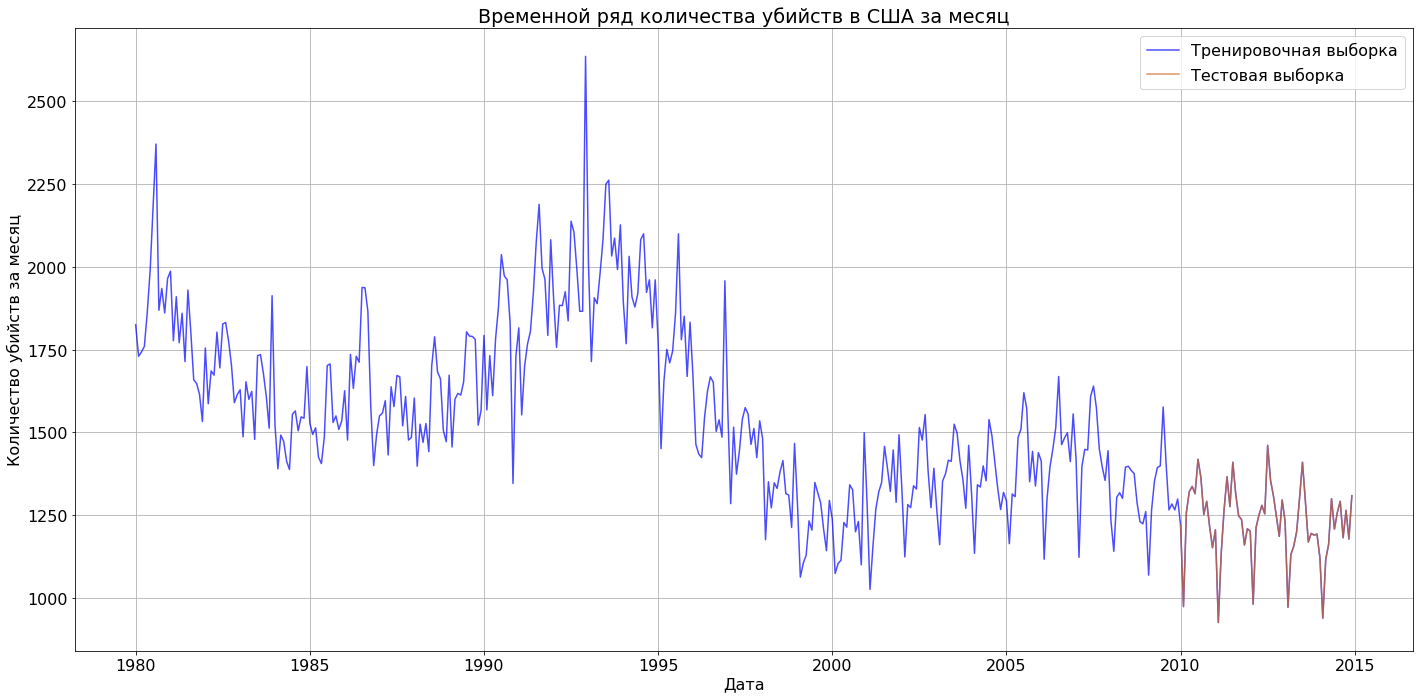
\includegraphics[scale=0.3]{time_series}}
        \captionsetup{labelformat=empty}
        \vspace{-2.3em}
        \caption[scale=0.25]{}
\end{figure}


\end{frame}

\begin{frame}
\frametitle{Применённые модели}
\begin{block}{\texttt{ElasticNet -- sklearn.linear\_model.ElasticNet}}
Подбор гиперпараметров с помощью \texttt{sklearn.linear\_model.ElasticNetCV}:\\
\texttt{l1\_ratio=[.01, .1, .5, .7, .9, .95, .99, .999, 1], n\_alphas=1000, max\_iter=10000}.\\
Лучшие значения для прогноза по 12 месяцам: l1\_ratio=0.1, alpha=3077.72.\\
Лучшие значения для прогноза по 24 месяцам: l1\_ratio=1, alpha=56.68.
\end{block}

\begin{block}{\texttt{MLP} -- фреймворк \texttt{PyTorch}}
Рассматривались архитектуры до четырёх полносвязных слоёв с батч-нормализацией и дропаутом. Лучшее качество достигнуто при использовании двухслойной архитектуры без батч-нормализации и дропаута.\\
Количество нейронов  нейронов скрытых слоёв: 12, 24, 32, 64, 96.\\
Лучшее значение: 32. Функция активации: \texttt{ReLU}.
\end{block}

\begin{block}{\texttt{RNN} и \texttt{LSTM} -- фреймворк \texttt{PyTorch}}
Размерность скрытого слоя: 16, 32, 64, 128, 256, 1024.\\
Лучшие значения для прогноза по 12 месяцам: 64. Лучшие значения для прогноза по 24 месяцам: 1024.
\end{block}

\begin{block}{\texttt{ARIMA} и \texttt{ARIMAX} -- пакет \texttt{statmodels}}
Произведено дифференцирование исходного ряда. Стационарность ряда проверена критерием Дики-Фуллера. Для выбора лучших параметров использовался критерий Акаике.\\
ARIMA --- order=(24, 1, 12). ARIMAX --- order=(12, 1, 0), seasonal\_order=(0, 0, 0, 0).
\end{block}


\end{frame}

\begin{frame}
\frametitle{Результаты экспериментов}

+features --- модель использует агрегированные признаки исходного набора данных

{\fontsize{7.5}{10}\selectfont {
\begin{table}
\centering
\caption{Метрики качества обученных моделей ElasticNet, MLP, LSTM на тестовой выборке}
\vspace{-5pt}
\begin{tabular}{|c|c|c|c|}
\hline
\  & \emph {RMSE} & \emph {Время обучения, с} & \emph {Время предсказания, с} \\
\hline
\emph {ElasticNet+features (12 месяцев)} & 74.17 & 0.15 & 0.00012 \\
\hline
\emph {MLP (12 месяцев)} & 70.16 & 32.1 (2092 эпохи) & 0.0002 \\
\hline
\emph {LSTM (12 месяцев)} & 76.45 & 44.1 & 0.001 \\
\hline
\emph {ElasticNet (24 месяца)} & 61.02 & 0.0016 & 0.00012 \\
\hline
\emph {MLP (24 месяца)} & 63.47 & 19.6 (1203 эпохи) & 0.0002 \\
\hline
\emph {LSTM (24 месяцев)} & 90.01 & 114.5 & 0.002 \\
\hline
\end{tabular}
\end{table}
}}

{\fontsize{7.5}{10}\selectfont {
\begin{table}
\centering
\caption{Метрики качества обученных моделей ARIMA и ARIMAX на тестовой выборке}
\vspace{-5pt}
\begin{tabular}{|c|c|c|c|}
\hline
\  & \emph {RMSE} & \emph {Время обучения, с} & \emph {Время предсказания, с} \\
\hline
\emph {ARIMA} & 64.92 & 2068.3 & 0.016 \\
\hline
\emph {ARIMAX} & 62.15 & 1.37 & 0.0076 \\
\hline
\end{tabular}
\end{table}
}}

\ \\
\textbf{Спецификации рабочих машин:} \\
\begin{itemize}
\item Измерение времени для \emph {ElasticNet} и \emph{MLP}: Intel Xeon E5-2699 v4 @ 2.20 ГГц, 12ГБ ОЗУ \\
\item Измерения времени для LSTM и RNN: Intel Core i-7-8750H @ 2.20ГГц, 16 ГБ ОЗУ, NVIDIA GeForce RTX 2060\\
\item Измерения времени для ARIMA и ARIMAX: Dual-Core Intel Core i5 @ 2.30ГГц, 8 ГБ ОЗУ\\
\end{itemize}

\end{frame}

\begin{frame}
\frametitle{Иллюстрация предсказаний лучшей модели ElasticNet}

\begin{figure}[h!]
        \center{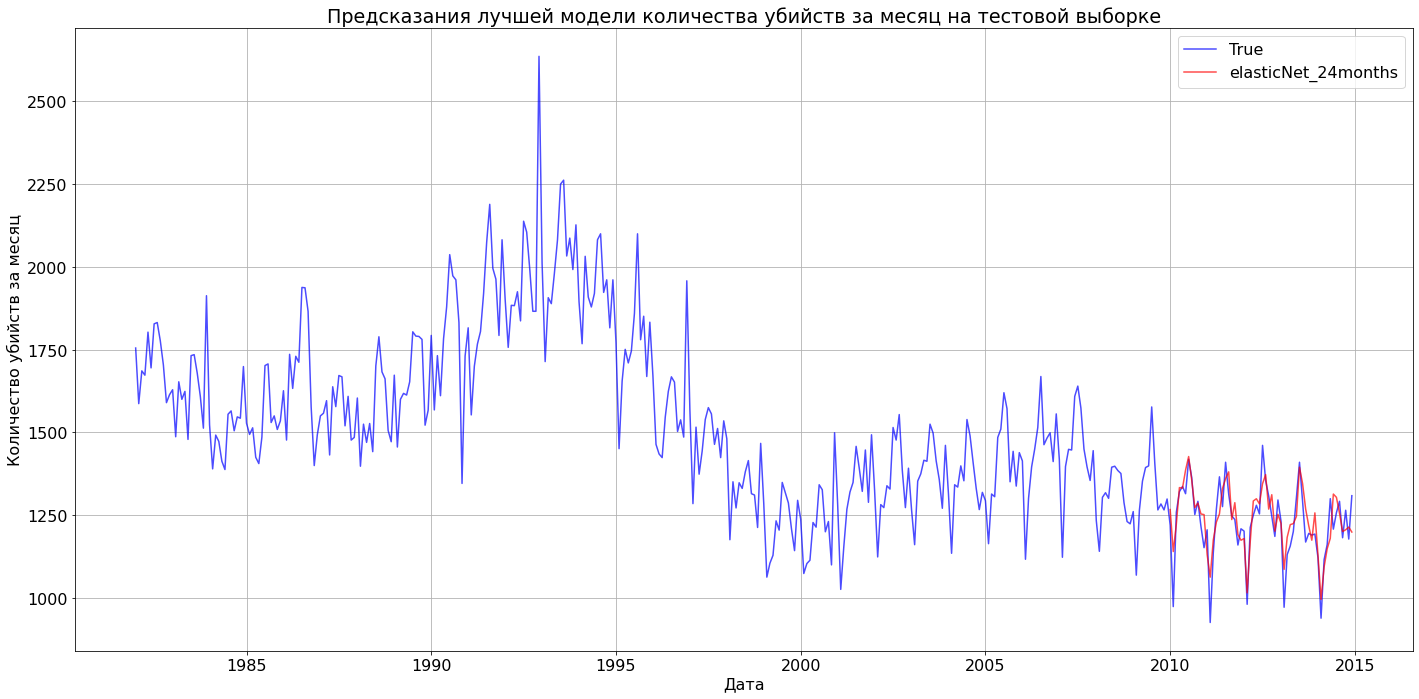
\includegraphics[scale=0.3]{elasticNet_24months}}
        \captionsetup{labelformat=empty}
        \vspace{-2.3em}
        \caption[scale=0.25]{}
\end{figure}
\end{frame}

\begin{frame}
\frametitle{Иллюстрация предсказаний лучшей модели ARIMAX}

\begin{figure}[h!]
        \center{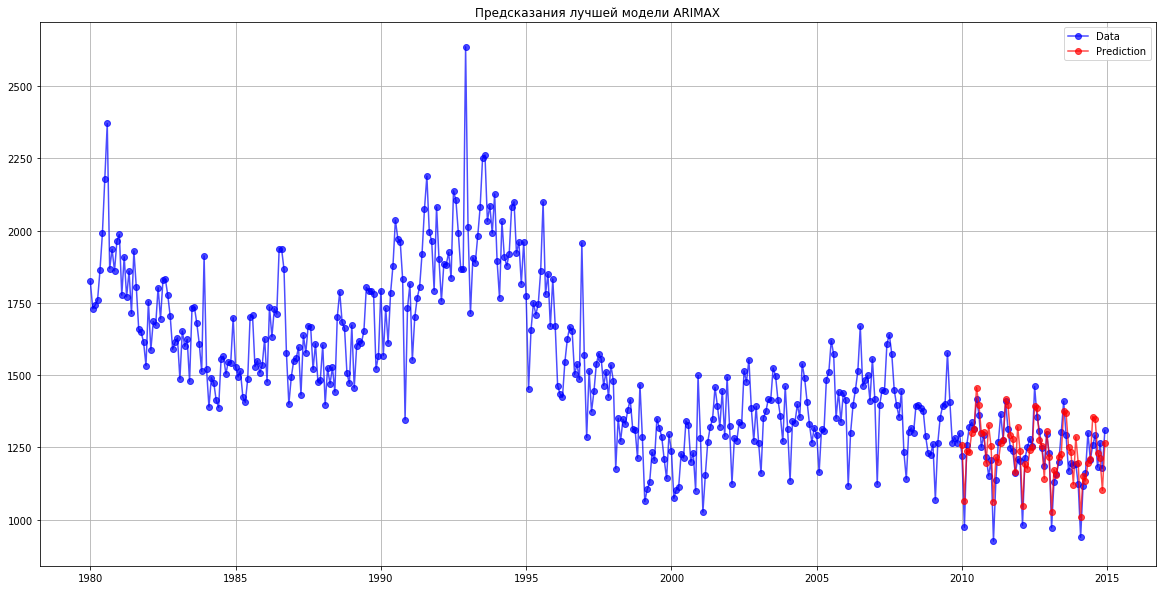
\includegraphics[scale=0.35]{arimax}}
        \captionsetup{labelformat=empty}
        \vspace{-2.3em}
        \caption[scale=0.25]{}
\end{figure}
\end{frame}

\end{document}
